\documentclass[12pt]{report}

\usepackage[top=3cm, bottom=3cm, left=3cm, right=3cm]{geometry}
\usepackage[T1]{fontenc} 
\usepackage[francais]{babel} %ecrire en français
\usepackage[utf8]{inputenc} 
\usepackage{graphicx}
\usepackage{hyperref}
\usepackage{pdfpages} 

\hypersetup{                    % parametrage des hyperliens
    colorlinks=true,                % colorise les liens
    breaklinks=true,                % permet les retours à la ligne pour les liens trop longs
    urlcolor= blue,                 % couleur des hyperliens
    linkcolor= blue,                % couleur des liens internes aux documents (index, figures, tableaux, equations,...)
    citecolor= green                % couleur des liens vers les references bibliographiques
    }
    
    
\begin{document}

\includepdf[scale = 1.4, pages=1]{PageGarde2.pdf}

\chapter*{Remerciements}
Ce stage de 2e année du cycle préparatoire a été réalisé dans l'entreprise Stimshop, située dans la pépinière d'entreprises de Paris Soleillet dans le 20e arrondissement. Cette première expérience professionnelle s'est déroulée sous la tutelle d'Arthur Aubertin, mon maître de stage, William Schlegel, le directeur technique de Stimshop et Dominique Palacci, le Président-directeur général de Stimshop. \\

Je tiens à adresser mes sincères remerciements à Arthur, mon maitre de stage, pour son implication à mon égard : il a fait de ce stage une expérience unique qui n'a cessé d'éveiller ma curiosité. Ses nombreux conseils m'ont permis d'en apprendre davantage et en profondeur sur de nombreux sujets. \\

Je souhaite également remercier William et Dominique pour leur bonne humeur et leur acharnement dans leur travail. \\

Je remercie également Mamed et JC pour leur accueil chaleureux, les journées de travail sans eux auraient sûrement paru beaucoup plus longues. Également très présents pour m'aider et me soutenir, ils ont répondu à beaucoup de mes interrogations. 
\newpage

\chapter*{Résumé}

Cette première expérience professionnelle chez Stimshop m'a permis de découvrir le travail au sein d'une jeune start-up tout en mettant en application mes connaissances en électronique, informatique ou même physique acquis à l'école. L'entreprise m'a également beaucoup appris sur le plan professionnel et relationnel. Les missions variées m'ont permis d'aiguiser mes connaissances dans de nombreux domaines principalement informatiques, avec l'apprentissage et l'application de nouveaux langages de programmation, mais aussi électroniques avec des applications telles que la conception de cartes électronique, de montage de boîtiers installés dans des magasins pour diffuser des ondes ultrasonores ou encore de multiples tests de distances des ondes pour plusieurs gammes de smartphones.
\newpage

\renewcommand{\contentsname}{Sommaire}
\tableofcontents

\chapter*{Introduction}

Etant passionné par les nouvelles technologies et innovations, j'ai choisi de réaliser mon stage de 2\ieme{} année du cycle préparatoire ingénieur dans une petite structure très porteuse dans le domaine de la transmission de données par ultrasons : Stimshop. Malgré la grande liberté laissée par l'ECE concernant le stage de 2e année, j'ai choisi de m'orienter vers un domaine qui m'intéresse beaucoup et en relation avec mon parcours d'ingénieur. 

\paragraph{}
je me suis rapidement orienté vers une petite structure dont l'organisation et le fonctionnement diffèrent d'une entreprise classique. Cet aspect d'organisation nouvelle et potentiellement rentable est très intéressant et peut amener à se demander si le fonctionnement d'une start-up permet une bonne cohésion et un bonne communication comparée à une entreprise de plus grande envergure. Mon réseau personnel m'a permis de m'orienter rapidement vers une Startup tournée mathématiques et algorithmie complexes. Je me suis alors rapidement rendu compte que cet objectif était au delà de mes compétences. Je me suis alors tourné vers un domaine plus familier :  l'interaction mobile. 

\paragraph{}
Ce domaine porteur qu'est l'interaction mobile, qui plus est via des ultrasons, m'a poussé à choisir Stimshop pour ce stage. Mes relations personnelles ont joué un rôle important dans la recherche de ce stage, malgré les nombreuses démarches personnelles, je n'ai reçu que peu de réponses positives de la part des recruteurs. Le domaine de l'interaction mobile et des ondes en général est en pleine expansion et également accessible à mon niveau de compétence : le développement logiciel, l'informatique ou encore l'électronique enseigné à l'école m'a aidé à travailler et à apprendre avec rigueur au sein de l'entreprise. La motivation de l'équipe de Stimshop m'a également permis de m'intégrer rapidement. 

\chapter{Description de l'entreprise}

	\section{Historique}
	
Stimshop est une société fondée en 2013 par Dominique Palacci, Thibaud Fayard, Jean Perret et Jérôme Gayet.\\

En 2009, un concept nommé "MobiStim" voit le jour. Il s'agit d'un concept d'animation des points de vente : une Borne MOBiSTiM installée sur le point de vente va communiquer par SMS, via un son spécifique, des informations (points de fidélité, réductions ciblées, etc.) aux mobiles dont le numéro a été saisi sur la borne. Cette technologie a l'avantage d'utiliser le son pour communiquer, ce qui lui permet d'être compatible avec tous les téléphones mobiles (tous équipés de microphone). Ce projet avait pour but de fidéliser les clients sur les points de ventes. \\
 
Cette première approche de la technologie sonore pour le retail (ou \href{https://www.insee.fr/fr/metadonnees/definition/c1647}{commerce de détail}) ajouté à la montée en puissance des smartphones à partir de 2012 va pousser Stimshop à se lancer dans l'interaction mobile par ultrasons. Afin de développer un signal ultrasonore exploitable, deux années de Recherches et Développement seront nécessaires. Le signal mis au point et breveté par stimshop est un signal ultrasonore ayant l'avantage d'être précis et utilisable partout (y compris là où les ondes radios ne sont pas autorisées ou utilisables : zones sécurisées, milieux explosifs, etc.). Les ondes ultrasonores ont l'avantage d'être très directives, ce qui est également un inconvénient puisque la surface couverte par l'onde sera très limitée, et le message envoyé ne pourra pas être très long (140 caractères maximum). Les smartphones actuels étant tous équipés de microphone, le signal stimshop à donc l'avantage d'être compatible avec tous les téléphones mobiles. \\

C'est à partir de la fin de l'année 2015 que Stimshop se lance sur le marché avec ses premières installations.\\ 

	\section{Organisation générale et organisation du service}

\begin{figure}[h!]
\begin{center}
\includegraphics[scale=0.5]{organigramme.PNG}
\end{center}
\caption{Organigramme de Stimshop}
\label{Organigramme de Stimshop}
\end{figure}

L'entreprise compte actuellement un salarié : Arthur Aubertin, responsable Recherche et développement, ingénieur doctorant en acoustique en possession d'un master en physique acoustique et d'une licence en ingénierie mécanique (UPMC), il est chez Stimshop depuis octobre 2016 et c'est lui qui s'occupe de la recherche et développement du signal Stimshop ainsi que du développement logiciel permettant l'interaction émetteur/récepteur pour le signal. Arthur est également responsable des stagiaires chez Stimshop. Mamed Kerrad et Jean-Christophe Melikian sont deux étudiants de l'ESGI en apprentissage chez Stimshop. Arrivés en septembre 2016, ils sont responsable du développement de l'application mobile et du SDK Stimshop. Mamed s'occupe du développement IOS (pour la technologie Apple) et Jean-Christophe s'occupe du développement de l'application pour la technologie Android. Ils développent dans leurs technologies respectives l'application "ucheck.in" et le SDK Stimshop Android. Le directeur technique de Stimshop est William Schlegel, ingénieur diplômé de l'EFREI et également président de l'entreprise Skrnz (interactions dans les salles de cinéma) et IglooSpirit (production et développement VR/AR). William est également enseignant à l'EFREI. Son rôle au sein de l'entreprise est de coordonner les travaux effectués par l'ingénieur (Arthur Aubertin) et les développeurs mobiles (Mamed Kerrad et Jean-Christophe Melikian). Dominique Palacci est le President directeur général et cofondateur de Stimshop, il s'occupe d'effectuer toutes les démarches commerciales de l'entreprise. L'effectif total de l'entreprise est de 5 personnes. L'organigramme de l'entreprise est disponible figure \ref{Organigramme de Stimshop}.

	\section{Politique commerciale}

Stimshop répond à plusieurs besoins dans deux domaines particuliers : le retail (ou \href{https://www.insee.fr/fr/metadonnees/definition/c1647}{commerce de détail}) et l'industrie.  Dans le domaine du retail, on retrouve du marketing de proximité avec l'envoi de messages commerciaux contextualisés pour les smartphones dans les points de vente (les ultrasons sont émis depuis les hauts-parleurs des magasins, à travers la musique d'ambiance), l'envoi de messages ciblés durant des événements, ou encore une détection de présence dans les universités par exemple. Dans le domaine de l'industrie, la principale utilité des signaux Stimshop se trouve dans l'émission et la réception de messages courts dans des endroits confinés où les ondes radio ne peuvent pas être transmises comme dans des centrales nucléaires par exemple. \\

Ayant déjà fait ses preuves dans le retail, Stimshop se concentre actuellement sur le domaine de l'industrie, afin de développer sur le long terme, une technologie capable de géolocaliser les smartphones via la technologie ultrasonore. \\

Stimshop base principalement son modèle économique sur la vente de licences mensuelles ou annuelles pour leur plate-forme et sur la vente de matériel. Les produits vendus par stimshop sont principalement des boîtiers qui émettent la technologie ultrasonore Stimshop. Ces boîtiers appelés HBeacon (Hybride Beacon) utilisent la technologie bluetooth en parallèle à la technologie Stimshop. L'entreprise vend également des boitiers nommés Umix dont le principal objectif est la détection de présence aux cours dans les universités Kedge. 

	\section{concurrents}

Au niveau de l'interaction et la communication de smartphone, Stimshop à trois concurrents directs : LISNR aux Etats-Unis, Copsonic en France, et Silverpush en Suède. Ces trois entreprises utilisent une technologie similaire pour transmettre des données : l'ultrason. La particularité de Stimshop est que leur signal joue sur la modulation linéaire de fréquence là où leurs concurrents jouent sur l'intensité du signal (similaire au morse). Le signal Stimshop permet également une multi-détection dans une même zone, absent chez les concurrents. 

	\section{partenaires}
		
Stimshop travaille en partenariat avec O'lab, qui produit et tient à jour les HBeacon. L'entreprise est également partenaire avec de nombreuses organisations telles que \href{https://www.orange-business.com/fr}{Orange Business Service}, \href{https://www.open.global/}{Open Group}, \href{https://worldline.com/content/worldline/en/home.html}{Wordline}, \href{https://swizi.open.global/}{Swizy by Open}, \href{https://www.mapwize.io/en/}{Mapwize}, \href{http://www.nomadicsolutions.biz/en/}{Nomadic Solutions}, Deep Block, \href{http://www.zento.fr/}{Zen'To}, \href{https://bealder.com/}{Bealder} ou encore \href{http://yppa.fans/}{Yppa}. 

	\section{Politique de ressources humaines}



\chapter{Missions et objectifs du stage}
		
Durant ce stage, de nombreuses missions m'ont été confiées, dans des domaines variés et à mon niveau de compétence. 

	\section{Assemblage et flashage des boitiers Umix}
		
\paragraph{}
Ma première mission au sein de Stimshop fut l'assemblage d'une trentaine de boîtiers appelé "Umix". Umix est un produit destiné à être vendu aux universités Kedge Business school. L'objectif de ces boîtiers est de détecter la présence des élèves de l'école assistants aux cours : lorsque le cours commence, la liste des élèves présents dans l'amphithéâtre s'affiche sur une tablette, permettant au professeur de faire un appel rapide pour compléter la liste en cas d'erreur. les boîtiers sont montés en quadrillage sur le plafond de chaque salle de classe et amphithéâtre pour diffuser et recevoir au mieux les ultrasons envoyés par les smartphones de chaque étudiant. Le fonctionnement de la technologie se résume simplement : lorsque le cours commence, le téléphone de chaque étudiant émet une onde ultrasonore qui sera récupérée par les boîtiers. L'onde associée à chaque étudiant sera ensuite envoyée à la tablette qui pourra confirmer leur présence au cours. L'avantage des ultrasons dans ce cas d'utilisation est que ces derniers ne traversent pas les murs contrairement aux ondes radio ou Wi-Fi. Cela permet une sorte d'étanchéité des salles de classe, évitant ainsi aux boîtiers de détecter des étudiants d'une autre salle ou d'être perturbés par le réseau extérieur.  

\begin{figure}[h!]
\begin{center}
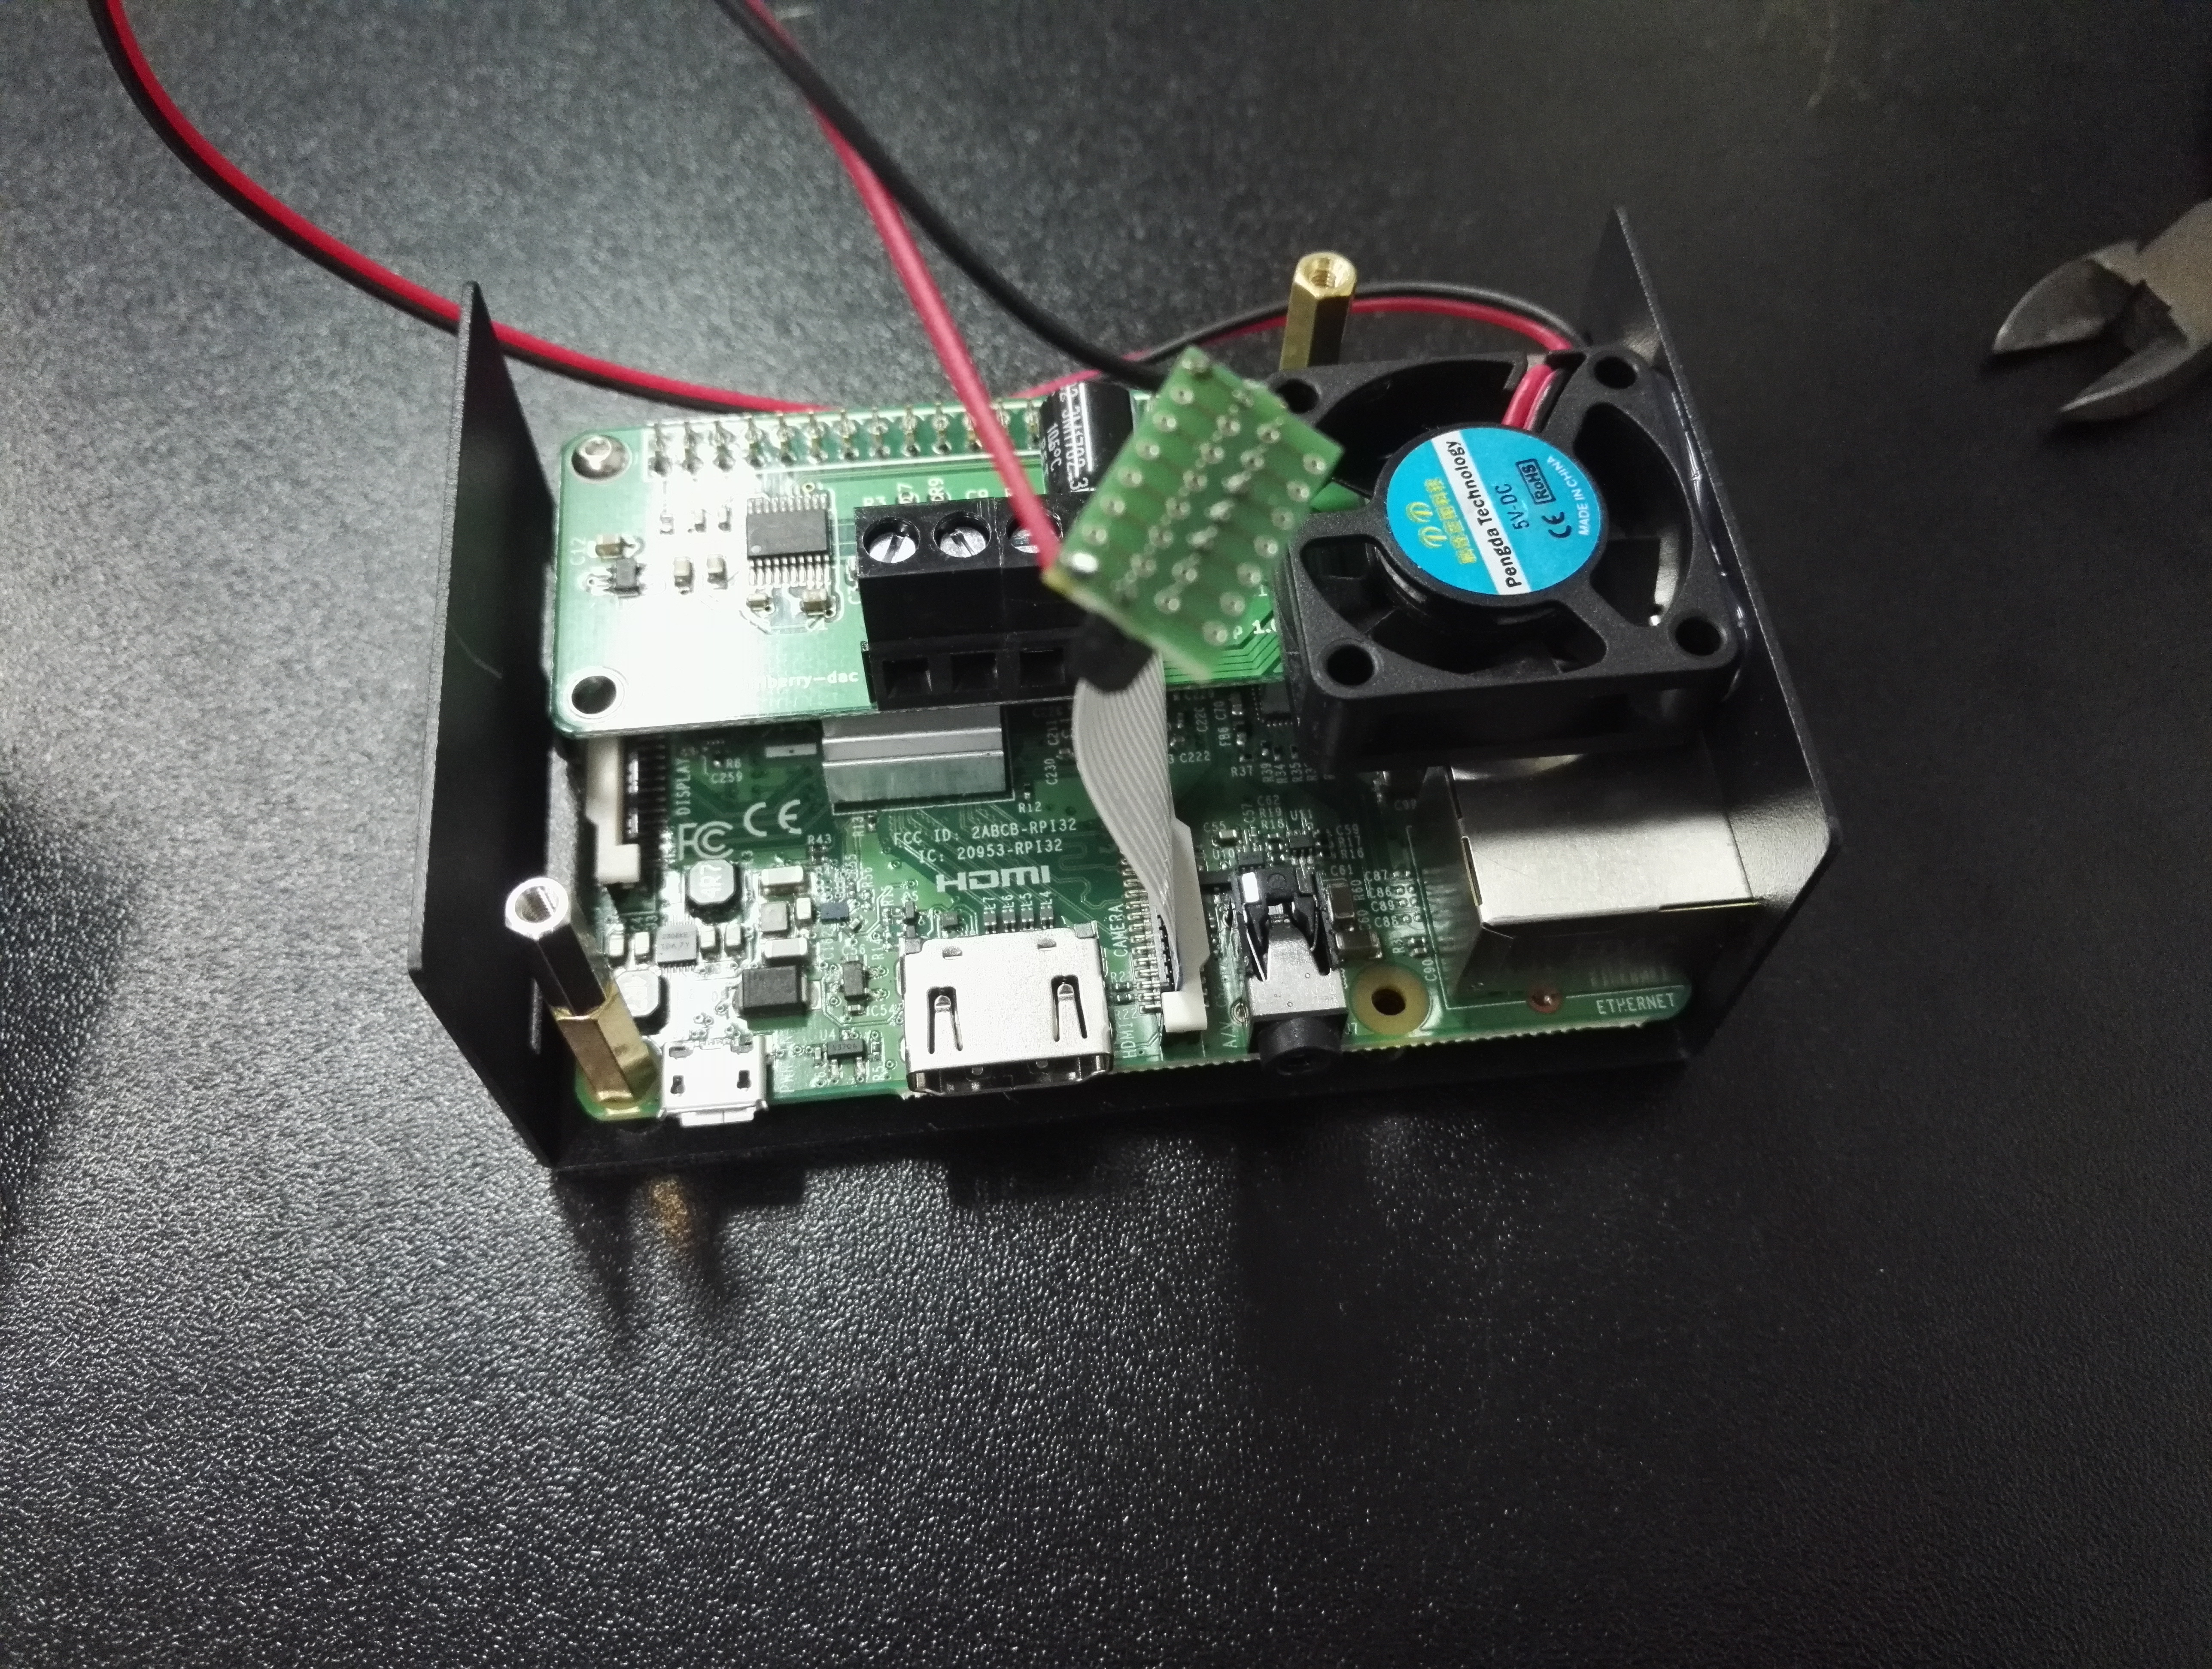
\includegraphics[scale=0.05]{Umix.jpg}
\end{center}
\caption{Intérieur d'un boîtier Umix}
\label{Intérieur d'un boîtier Umix}
\end{figure}

\paragraph{}
La technologie Umix est contrôlée par un Raspberry Pi associé à un module directement connecté à deux ports RCA. Un ventilateur connecté au raspberry via une nappe permet de refroidir la carte. 

\paragraph{}
Ma mission concernant ces boîtiers fut manuelle : visser le Raspberry et le module au boîtier, puis connecter le ventilateur au Raspberry via une nappe et un connecteur adaptateur particulier, coller le ventilateur au boîtier et enfin fermer et visser le boîtier. Un travail de soudure/dessoudure a également été nécessaire dû à des fils trop courts (soudés au RCA), ou mal soudés en amont. Ce travail répétitif m'a permis de prendre la main assez rapidement pour assembler à la chaîne ces 30 boîtiers Umix dont un modèle est donné en figure \ref{Interieur d'un boîtier Umix}.  

\paragraph{}
Ma seconde mission fut de "flasher" les Raspberry de chaque boîtier, c'est-à-dire mettre à jour le micrologiciel des Raspberry pour qu'ils fonctionnent correctement. Cette étape consistait simplement à graver l'image disque envoyée par Kedge (le micrologiciel à jour) sur une carte micro SD insérée dans le Raspberry. Une fois l'image gravée, il fallait tester le bon fonctionnement de chaque boîtier en les connectant à un ordinateur et en saisissant le nom d'utilisateur et le mot de passe envoyé par Kedge. 
Cette mission n'a nécessité que peu de compétences spécifiques, mais une bonne gestion du temps était primordiale : une fois l'image reçue, la livraison devait être prête pour le lendemain. Il me fallait donc flasher 30 Raspberry en une journée. Sachant qu'il fallait environ 20 minutes pour flasher un Raspberry, deux ordinateurs tournant en continu furent nécessaires. Finalement, les boîtiers étaient prêts à temps pour la livraison, seul un boîtier sur les trente était "défectueux" car très bruyant, un remplacement du ventilateur fut nécessaire. Cette première mission plutôt manuelle, m'a appris à être minutieux et optimisé dans mon travail à la chaîne, le délai de livraison à respecter m'a également appris qu'être organisé dans son travail est essentiel. 

	\section{Conception d'une carte électronique sous Eagle}

\begin{figure}[h!]
\begin{center}
\includegraphics[scale=0.05]{Hbeacon.jpg}
\end{center}
\caption{Le HBeacon de Stimshop}
\label{Le HBeacon de Stimshop}
\end{figure}

Le principal produit créé par stimshop s'appelle HBeacon (pour Hybride Beacon). Le HBeacon permet d'envoyer un signal stimshop (ultrasonore) via une pastille piézoélectrique (informations techniques complémentaires \href{https://fr.wikipedia.org/wiki/Pi%C3%A9zo%C3%A9lectricit%C3%A9}{ici}) contrôlée par une carte électronique. 
Installé en hauteur dans des magasins, le HBeacon va envoyer aux smartphones des clients des messages commerciaux, points de fidélité, etc. via les ultrasons Stimshop. 
Comme les boîtiers Umix, le HBeacon nécessite d'être flashé pour fonctionner correctement. Mais le Hbeacon n'est pas un simple Raspberry : c'est une carte électronique fait sur mesure pour les besoins de stimshop sans aucun connecteurs. Comme montré sur la figure \ref{Le HBeacon de Stimshop}, le HBeacon est grossièrement constitué d'un emplacement pour une pile plate (à l'arrière), d'une antenne bluetooth (permettant de s'y connecter pour le paramétrer), et d'une pastille piézoélectrique (permettant d'émettre le signal ultrasonore). 

\paragraph{}
Il n'est pas possible de connecter le HBeacon à un ordinateur via un câble USB lambda ou une carte SD, un adaptateur MiniProg3 est nécessaire. La connectique de la carte étant placée dans un ordre différent de celle de l'adaptateur, une carte électronique faisant office d'adaptateur était nécessaire pour simplifier la connexion et éviter les fils. 
Ma mission tout d'abord fut la prise en main du logiciel Eagle, un logiciel de conception de circuit imprimé. Aidé par Arthur, il m'a fallu une journée pour prendre en main le logiciel. 
L'objectif de ma mission consistait en la conception d'une carte adaptateur fonctionnelle permettant de connecter le HBeacon au MiniProg3. Pour ce faire, 5 trous et via de chaque côté de la carte pour les 5 connecteurs du Hbeacon et du MiniProg3 devaient être reliés via des pistes sur le côté cuivre de la carte. Il me fallait également choisir les connecteurs à pins a insérer dans ces trous : mâle/femelle d'un côté, et mâle/mâle de l'autre. Pour concevoir la carte, de nombreuses contraintes devaient être respectées : diamètre des trous et via suivants le connecteur choisi, largeur des pistes, espace entre les vias suivant l'espace entre les pins du connecteur choisi, taille de la carte ou encore la sérigraphie. N'ayant aucune expérience avec ce genre de logiciel, la carte paraissant plutôt simple à concevoir sur le papier ne s'est pas faite sans difficulté, notamment pour la gestion des couches (avec une utilisation particulière pour chacune), ou encore pour relier les vias ensemble via les pistes.
Une fois la carte manufacturée et les connecteurs reçu, il restait simplement à souder les 5 pins de chaque connecteur dans les 5 trous de la carte. L'adaptateur final fonctionnel est présent en figure \ref{Adaptateur Hbeacon vers MiniProg3}.

\begin{figure}[h!]
\begin{center}
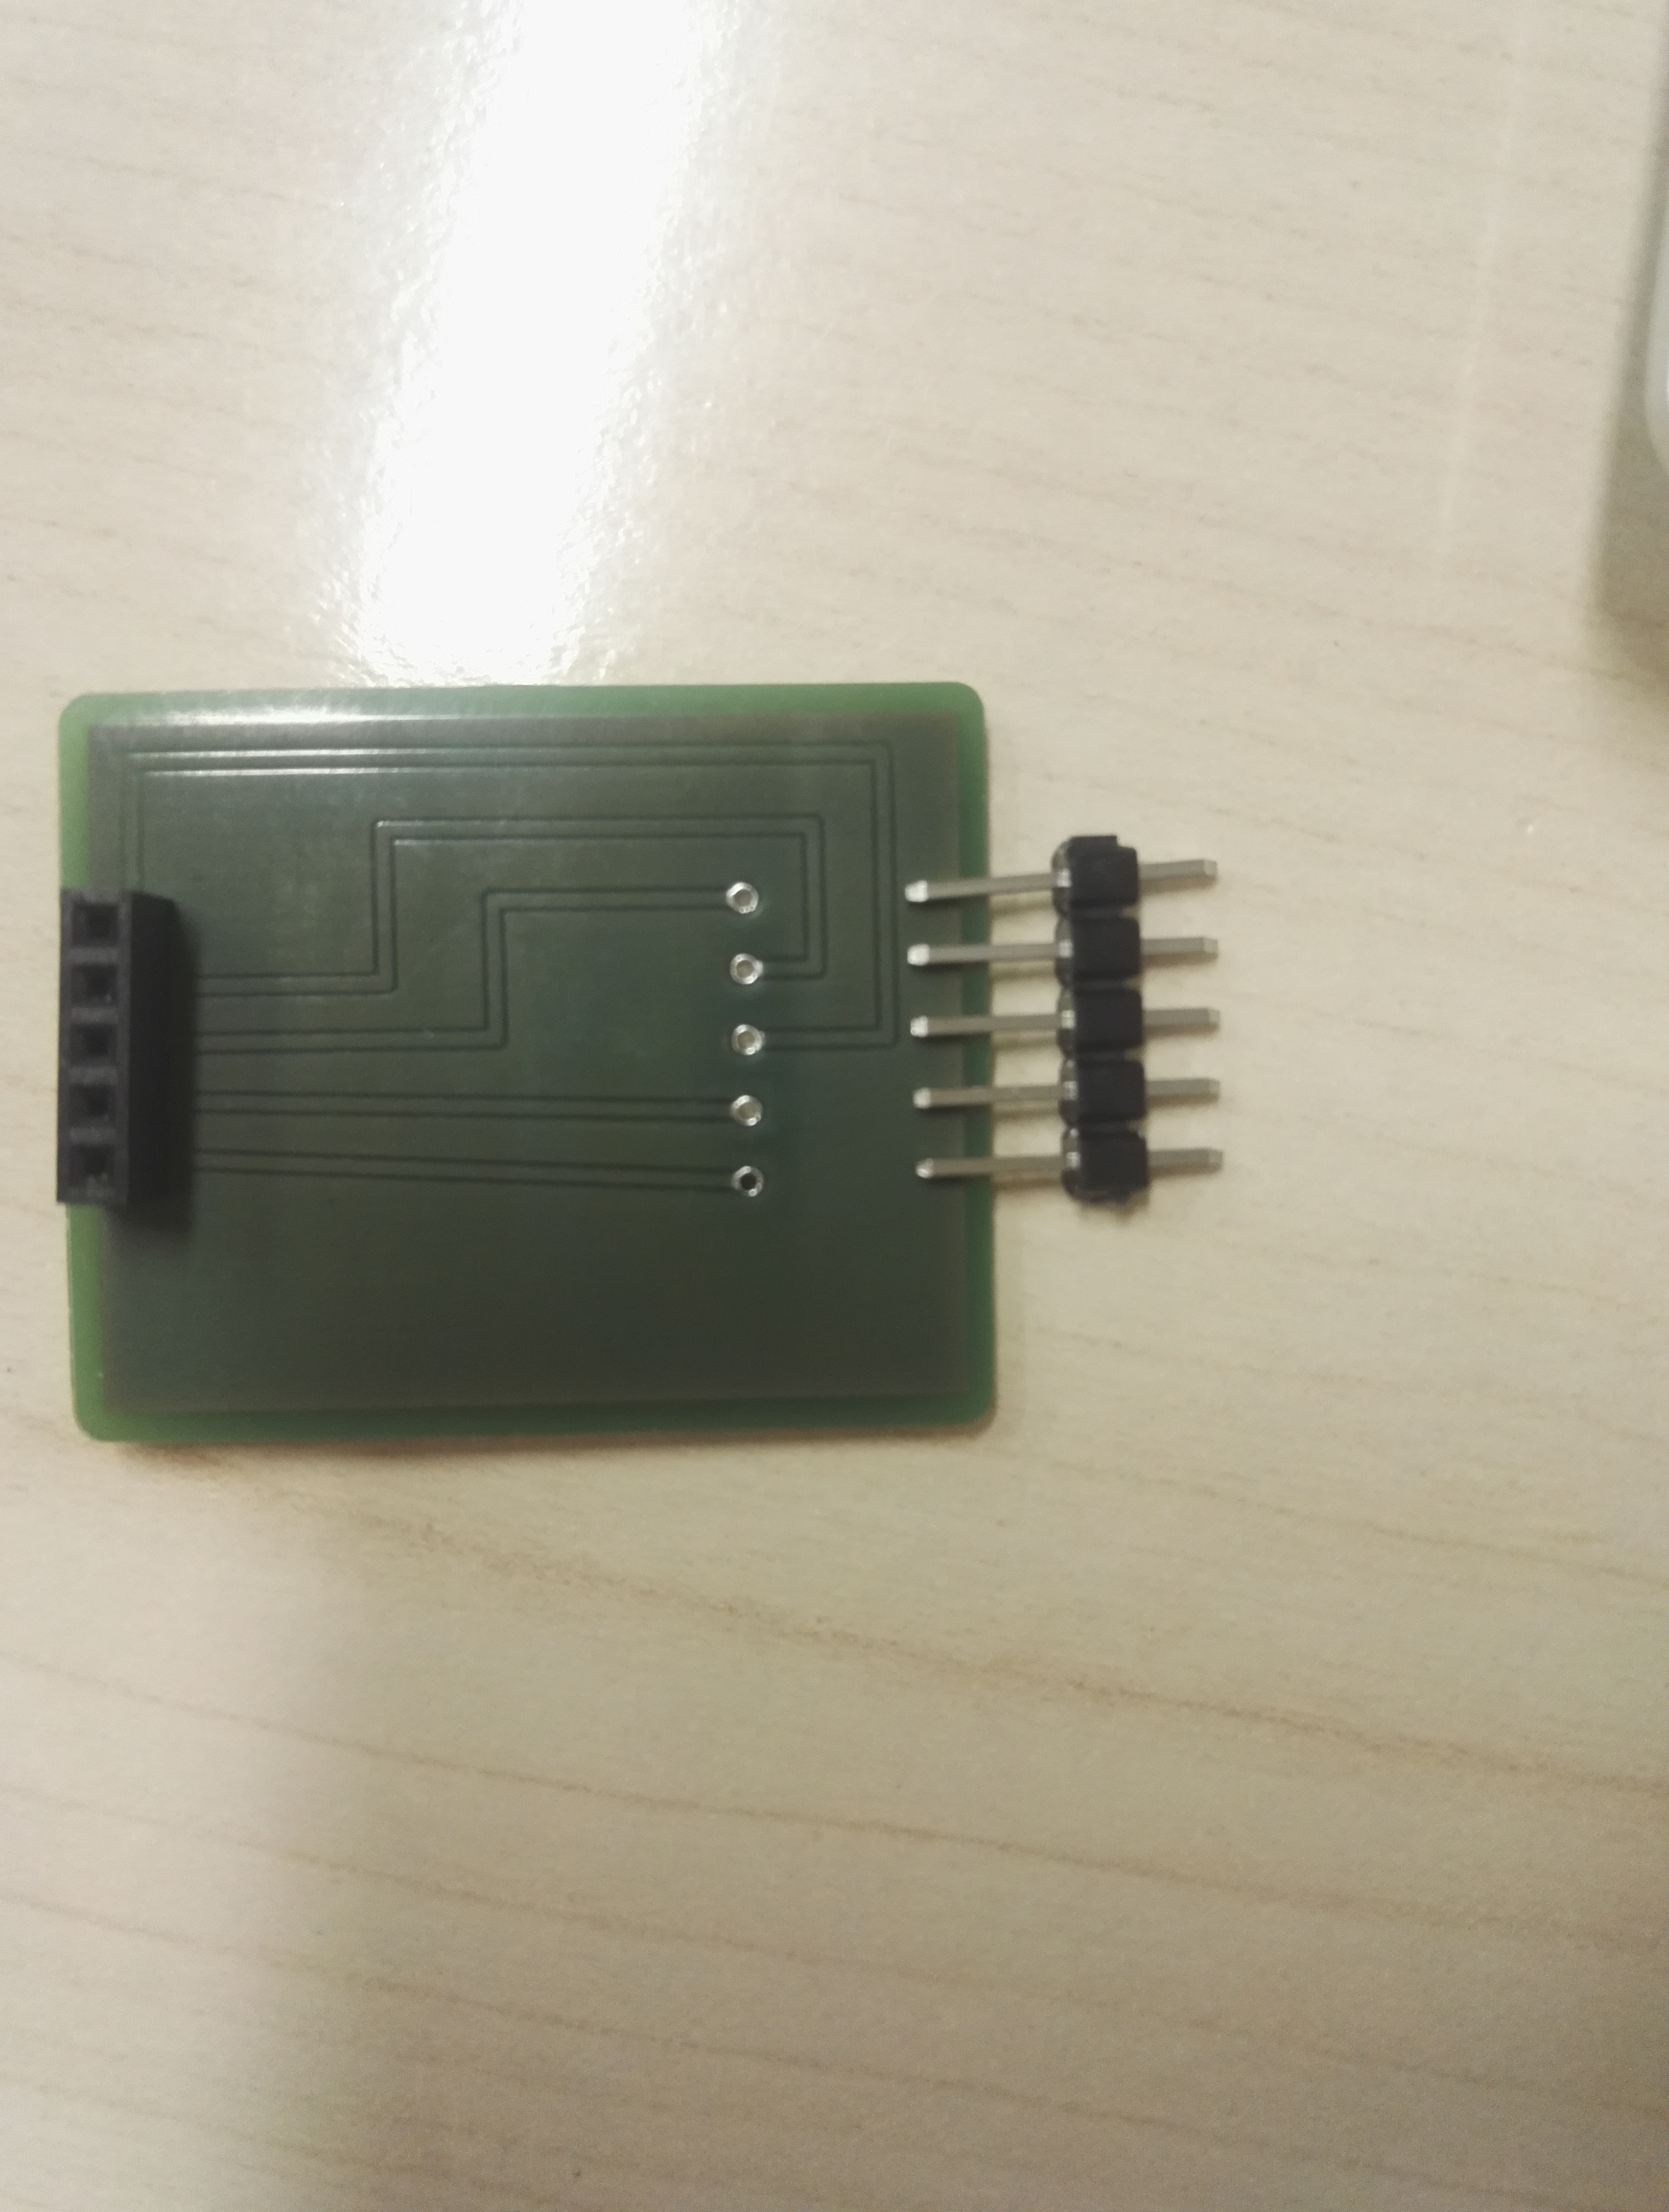
\includegraphics[scale=0.05]{Adapter2.jpg}
\end{center}
\caption{Adaptateur Hbeacon vers MiniProg3}
\label{Adaptateur Hbeacon vers MiniProg3}
\end{figure}

Cette première expérience technique m'a permis d'apprendre à utiliser le logiciel Eagle afin d'obtenir un résultat concret et fonctionnel. Le coût de production d'une carte à l'unité étant très cher, il me fallait être rigoureux dans mon travail pour être productif. J'ai également pu mettre en application des connaissances théoriques et pratiques vues à l'école, notamment en électronique : l'utilisation de logiciel de simulation de circuit comme ISIS Proteus ou encore Pspice m'a permis d'être plus à l'aise sur Eagle, logiciel nécessitant un schéma électrique du circuit en amont avant de passer à la carte en elle-même. La soudure des pins sur la carte était également un travail minutieux car très proche les unes des autres.

\paragraph{}
Après m'avoir envoyé un modèle de mixeur passif sur breadboard, Arthur m'a chargé de faire ce schéma sous Eagle afin d'en faire une carte électronique. Il m'a d'abord fallu dessiner à la main un schéma selon le circuit sur BreadBoard afin d'en comprendre le sens. Le circuit sur BreadBoard étant un peu volumineux, il m'a fallu un certain temps pour le comprendre et le retranscrire correctement sous la forme d'un schéma plus concret. Une fois le schéma dessiné, il ne restait plus qu'à le dessiner sous Eagle avec les bons composants, puis ajouter le routage entre tous les éléments du circuit. 

\paragraph{}
La partie la plus compliquée pour concevoir cette carte fut l'analyse et la compréhension du circuit sur BreadBoard. Mes connaissances en électronique et les nombreux TPs effectués sur BreadBoard à l'école m'ont aidé à comprendre le fonctionnement du schéma étudié ici. En revanche, la partie sur logiciel s'est faite sans problème. 

	\section{Mesures expérimentales des technologies Stimcom et Stimshop}

Le signal StimCom est dérivé de la technologie Stimshop : sa portée est supérieure et il peut envoyer plus d'informations. Stimcom est actuellement utilisé pour le projet Gravelines, consistant à la communication en interne de la centrale nucléaire de Gravelines. En effet, les ondes radio pouvant poser plusieurs problèmes dans les centrales nucléaires, les ultrasons sont une fin à la communication. 
Ma mission était de réaliser une série de mesures de puissance sonore du signal StimCom (en dB) émis depuis une valise RDK (utilisée pour le projet Gravelines). J'ai donc réalisé ces mesures à l'aide d'un sonomètre et noté les résultats selon la puissance du signal (un potentiomètre permet d'amplifier le signal) afin de dresser un rapport à Arthur. 
Cette mission ne nécessitait aucune compétence en particulier, mais il est toujours intéressant de connaître le fonctionnement de la valise RDK et de la technologie StimCom. Cela m'a également appris à rédiger un rapport résumant les mesures effectuées.\\

J'ai ensuite effectué des mesures de portées du signal Stimshop émis par un HBeacon. Aidé par Arthur, j'ai mesuré la portée du signal Stimshop en fonction du canal de fréquence choisi : le premier canal utilisé par Stimshop se situe entre 18kHz et 19kHz, le dernier canal (canal 3) se situe entre 20kHz et 21kHz. Le signal est reçu par le microphone d'un smartphone via un message de 5 caractères hexadécimaux. Suivant la puissance du smartphone récepteur, le signal peut être plus ou moins bien reçu. Après avoir effectué les mesures, j'ai pu en déduire que le canal 3 permet une grande portée du signal et qu'un smartphone nouvelle génération peut recevoir l'onde jusqu'à 15 mètres de distance. J'ai également effectué des mesures en cône pour connaître la surface au sol couverte par l'onde. L'ultrason étant une onde très directive, cette dernière ne peut s'étendre sur plus de deux mètres. 

	\section{Etude et modifications de code en C} 

Afin de générer un signal Stimshop au format .WAV, un programme codé en langage C est nécessaire. Ce programme permet notamment de créer un signal d'une minute en saisissant la fréquence souhaitée et les caractères hexadécimaux à envoyer en paramètre. Pour information, le signal Stimshop utilise plusieurs canaux de fréquences qui s'étendent de 17kHz à 21kHz et il peut envoyer jusqu'à 5 caractères hexadécimaux.  
Ma première mission consistait à analyser ce code afin de générer un fichier audio .wav puis le visualiser. Les bases en langage C acquises à l'école furent très utiles pour l'étude de ce programme, mais il m'a fallu un certain temps avant de le comprendre dans son intégralité. En effet, certains aspects assez techniques m'ont poussé à poser plusieurs questions à Arthur, mon maître de stage, notamment concernant le fenêtrage du signal. Pour comprendre ce programme, il m'a fallu analyser minutieusement chaque variable de chaque sous-programme pour en comprendre la logique. 

\chapter{Réflexions et critiques du monde du travail}



\chapter*{Conclusion}

\includepdf[scale = 1.1, pages=1]{fiche_eval.pdf}

\end{document}
